
\begin{figure}
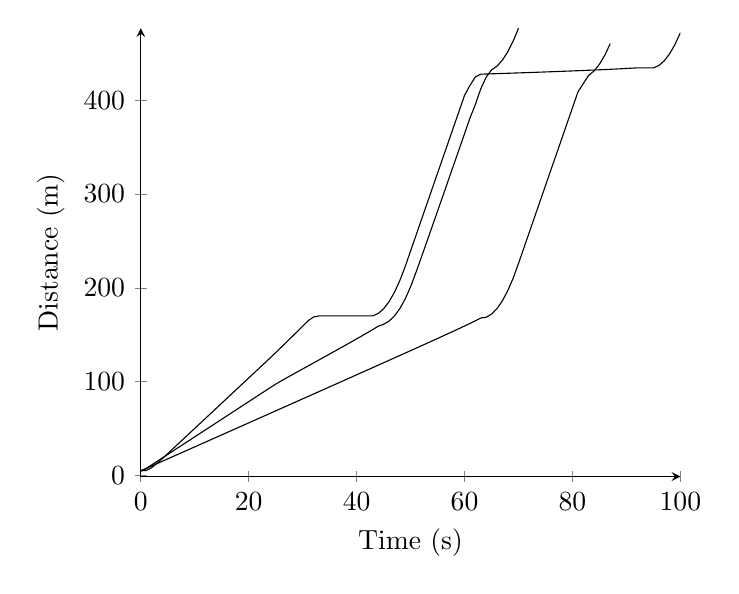
\begin{tikzpicture}
\begin{axis}[
legend style={anchor=west},
axis x line=bottom,
axis y line=left,
ymin=-1,
xlabel=Time (s),
ylabel=Distance (m),
]
\addplot[] coordinates {
(0, 5.1)
(1, 7.6)
(2, 10.1552443813)
(3, 12.7105738385)
(4, 15.2659922742)
(5, 17.8215038339)
(6, 20.377112925)
(7, 22.9328242377)
(8, 25.4886427682)
(9, 28.0445738441)
(10, 30.6006231525)
(11, 33.1567967706)
(12, 35.7131012)
(13, 38.2695434045)
(14, 40.8261308516)
(15, 43.3828715595)
(16, 45.9397741485)
(17, 48.496847899)
(18, 51.0541028157)
(19, 53.6115497)
(20, 56.1692002311)
(21, 58.7270670571)
(22, 61.2851638979)
(23, 63.8435056615)
(24, 66.4021085755)
(25, 68.9609903372)
(26, 71.5201702838)
(27, 74.0796695877)
(28, 76.6395114804)
(29, 79.1997215091)
(30, 81.7603278342)
(31, 84.321361573)
(32, 86.8828572)
(33, 89.4448530139)
(34, 92.0073916849)
(35, 94.5705208998)
(36, 97.1342941252)
(37, 99.6987715147)
(38, 102.264020994)
(39, 104.830119565)
(40, 107.397154884)
(41, 109.965227184)
(42, 112.534451629)
(43, 115.104961227)
(44, 117.676910452)
(45, 120.250479801)
(46, 122.825881573)
(47, 125.400088237)
(48, 127.976689677)
(49, 130.555966937)
(50, 133.138436412)
(51, 135.724640039)
(52, 138.315252314)
(53, 140.91112443)
(54, 143.513347807)
(55, 146.123348025)
(56, 148.743028237)
(57, 151.374996682)
(58, 154.022945018)
(59, 156.692315908)
(60, 159.391575704)
(61, 162.134911251)
(62, 164.948899855)
(63, 167.89373682)
(64, 168.705135954)
(65, 172.016535087)
(66, 177.827934221)
(67, 186.139333355)
(68, 196.950732488)
(69, 210.262131622)
(70, 226.073530756)
(71, 242.673530756)
(72, 259.273530756)
(73, 275.873530756)
(74, 292.473530756)
(75, 309.073530756)
(76, 325.673530756)
(77, 342.133530756)
(78, 358.733530756)
(79, 375.333530756)
(80, 391.933530756)
(81, 408.533530756)
(82, 417.63158871)
(83, 426.457948192)
(84, 431.130559011)
(85, 438.30316983)
(86, 447.97578065)
(87, 460.148391469)
};
\addplot[] coordinates {
(0, 5.1)
(1, 5.46690514645)
(2, 8.33381029291)
(3, 13.2342022663)
(4, 18.1229068485)
(5, 23.4862626488)
(6, 28.8498592741)
(7, 34.213722776)
(8, 39.5778831093)
(9, 44.9423748935)
(10, 50.3072383586)
(11, 55.672520532)
(12, 61.038276741)
(13, 66.4045725318)
(14, 71.7714861499)
(15, 77.1391117807)
(16, 82.5075638396)
(17, 87.8769827315)
(18, 93.2475427055)
(19, 98.6194627542)
(20, 103.99302204)
(21, 109.368582219)
(22, 114.746620569)
(23, 120.127780643)
(24, 125.512952386)
(25, 131.003256489)
(26, 136.600517425)
(27, 142.207762118)
(28, 147.829769131)
(29, 153.475085827)
(30, 159.160935073)
(31, 164.92955101)
(32, 168.903787215)
(33, 170.100630511)
(34, 170.218835629)
(35, 170.218835629)
(36, 170.218835629)
(37, 170.218835629)
(38, 170.218835629)
(39, 170.218835629)
(40, 170.218835629)
(41, 170.218835629)
(42, 170.218835629)
(43, 170.218835629)
(44, 172.718835629)
(45, 177.718835629)
(46, 185.218835629)
(47, 195.218835629)
(48, 207.718835629)
(49, 222.718835629)
(50, 239.318835629)
(51, 255.918835629)
(52, 272.518835629)
(53, 289.118835629)
(54, 305.718835629)
(55, 322.318835629)
(56, 338.778835629)
(57, 355.378835629)
(58, 371.978835629)
(59, 388.578835629)
(60, 405.178835629)
(61, 415.702018716)
(62, 424.685201803)
(63, 427.668384889)
(64, 427.859053032)
(65, 428.050928262)
(66, 428.244082531)
(67, 428.438594366)
(68, 428.634549713)
(69, 428.832042924)
(70, 429.031177914)
(71, 429.232069531)
(72, 429.434845188)
(73, 429.639646813)
(74, 429.846633209)
(75, 430.055982922)
(76, 430.267897763)
(77, 430.482607177)
(78, 430.700373708)
(79, 430.921499935)
(80, 431.146337378)
(81, 431.375298101)
(82, 431.608870084)
(83, 431.84763797)
(84, 432.092311664)
(85, 432.343766748)
(86, 432.603103247)
(87, 432.871734041)
(88, 433.151523453)
(89, 433.445015695)
(90, 433.755836094)
(91, 434.08945643)
(92, 434.401866654)
(93, 434.401866654)
(94, 434.401866654)
(95, 434.401866654)
(96, 436.901866654)
(97, 441.901866654)
(98, 449.401866654)
(99, 459.401866654)
(100, 471.901866654)
};
\addplot[] coordinates {
(0, 5.1)
(1, 7.6)
(2, 11.3437025016)
(3, 15.0875902316)
(4, 18.8316758814)
(5, 22.5759733301)
(6, 26.3204977873)
(7, 30.0652659565)
(8, 33.8102962233)
(9, 37.5556088734)
(10, 41.3012263443)
(11, 45.0471735192)
(12, 48.7934780703)
(13, 52.5401708614)
(14, 56.2872864224)
(15, 60.034863512)
(16, 63.7829457867)
(17, 67.5315826014)
(18, 71.2808299736)
(19, 75.0307517494)
(20, 78.7814210256)
(21, 82.5329218935)
(22, 86.2853515939)
(23, 90.0388232032)
(24, 93.7934690071)
(25, 97.4620806134)
(26, 100.817082221)
(27, 104.054684782)
(28, 107.251536893)
(29, 110.435546622)
(30, 113.616742707)
(31, 116.798886597)
(32, 119.980874523)
(33, 123.165443138)
(34, 126.354141868)
(35, 129.548208386)
(36, 132.748995355)
(37, 135.958216755)
(38, 139.178190904)
(39, 142.412189133)
(40, 145.665026971)
(41, 148.94417199)
(42, 152.262051126)
(43, 155.641617148)
(44, 159.133389674)
(45, 161.223562664)
(46, 164.584505285)
(47, 169.978046551)
(48, 177.871587817)
(49, 188.265129082)
(50, 201.158670348)
(51, 216.552211614)
(52, 232.723715341)
(53, 249.010876058)
(54, 265.382098738)
(55, 281.81459597)
(56, 298.291850367)
(57, 314.801846202)
(58, 331.33581972)
(59, 347.747366901)
(60, 364.311801618)
(61, 380.885691346)
(62, 395.391900065)
(63, 411.991900065)
(64, 424.458551067)
(65, 432.293918326)
(66, 436.162706503)
(67, 442.531494681)
(68, 451.400282858)
(69, 462.769071035)
(70, 476.637859212)
};

\end{axis}
\end{tikzpicture}
\label{tik:distance:100:28}
\caption{100 percent diving with GSC on route $28$}
\end{figure}
